\apendice{Documentación técnica de programación}
\section{Introducción}
En esta parte del anexo pasaremos a ver de qué manera se halla organizado el proyecto con su estructura de directorios y archivos, también veremos todo aquello fundamental para la instalación del proyecto y poder ejecutarlo o trabajar con ello. También se verá la manera en qué se compila y se ejecuta, todo ello con documentación gráfica sobre los procesos. 

A parte de aquellos requerimientos que sean especificados a lo largo de este apéndice, también será fundamental para usarlo o trabajar con ello conocimientos específicos tanto de Unity como de C\#.

\section{Estructura de directorios}
El directorio del proyecto es el que se muestra a continuación, aunque pueda contener variaciones debido a temas de confidencialidad:
\begin{itemize}
\item \textbf{Proyecto/Assets} En esta carpeta se hayan contenidos todos los ficheros relacionados con las escenas, scripts y plugins añadidos.	
\begin{itemize}
    \item \textbf{/Assets/Art} Carpeta que contiene el arte utilizado en el proyecto.
    \item \textbf{/Assets/MyScripts} Carpeta que contiene los Scripts desarrollados para el proyecto.
    \item \textbf{/Assets/Oculus} Carpeta derivada de la descarga del plugin de Oculus para Unity.
    \item \textbf{/Assets/Prefabs} Carpeta que contienen objetos de las escenas.
    \item \textbf{/Assets/Resources} 
    \item \textbf{/Assets/RobotConnector} Carpeta que contiene Scripts para el trabajo con el robot.
    \item \textbf{/Assets/ROSBridgeLib-master} Carpeta con librerías que sirven de puente entre ROS y Unity.
    \item \textbf{/Assets/Scenes} Carpeta que contiene las escenas desarrolladas por mi en el proyecto. Es la carpeta que contiene desde los pequeños resultados que se iban consiguiendo, hasta la escena \textit{Ros} con el software final.
    \item \textbf{/Assets/SenseGlove} Carpeta que contiene las librerías para el uso de SenseGlove Nova en Unity.
    \item \textbf{/Assets/TextMesh Pro} Carpeta derivada de la instalación del plugin TextMeshPro.
    \item \textbf{/Assets/XR} Carpeta derivada de la instalación del plugin XR.
    
\end{itemize}
\item\textbf{Proyecto/Library} En esta carpeta se hayan contenidas las librerías de las que dispone Unity.
\item\textbf{Proyecto/Logs} En esta carpeta se contienen logs(registros).
\item\textbf{Proyecto/obj} 
\item\textbf{Proyecto/Packages} Carpeta que contiene datos sobre los paquetes instalados en Unity.
\item\textbf{Proyecto/ProjectSettings} Carpeta que contiene información sobre la configuración de proyecto.
\item\textbf{Proyecto/Temp} Carpeta que contiene archivos temporales.
\item\textbf{Proyecto/UserSettings} Carpeta que contiene configuración del usuario.
\end{itemize}

\newpage
\section{Manual del programador}
En esta sección prepararemos nuestro entorno de cara a poder compilar, instalar y ejecutar el proyecto en sí. Para ello veremos qué instalaciones son requeridas para el correcto trabajo, los pasos necesarios y aquellos requerimientos de PC destacados. 
En primer lugar vemos los requisitos mínimos y recomendados de Unity para ser instalado y que funcione correctamente:

\begin{figure}[h]
\centering
\label{Requisitos mínimos y recomendados Unity}
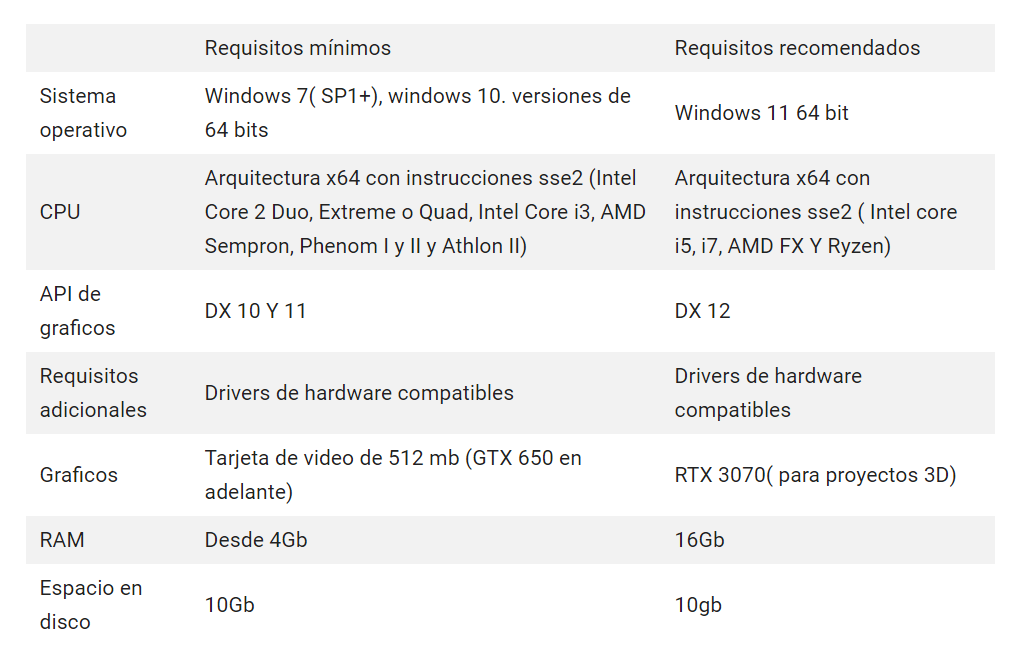
\includegraphics[width=\textwidth]{img/unity req.PNG}
\caption{Requisitos mínimos y recomendados Unity \cite{Requerimientos}}
\end{figure}

\subsubsection{Instalando Unity}
Para comenzar con la instalación es necesario acceder a su página web, donde debemos registrarnos y seleccionar el tipo de cuenta por la licencia de uso y se nos descargará el ejecutable UnityHub en su última versión (La 3.1.2 actualmente).

Deberemos de seleccionar el lugar de instalación de este programa que nos permitirá gestionar nuestros proyectos.
Después, se nos abrirá una ventana del Unity Hub donde en el apartado de Projects podremos en un futuro ver qué proyectos tenemos, vamos a la pestaña de instalaciones y veremos lo siguiente:

\newpage
\begin{figure}[h]
\centering
\label{Instalación Editor Unity 1}
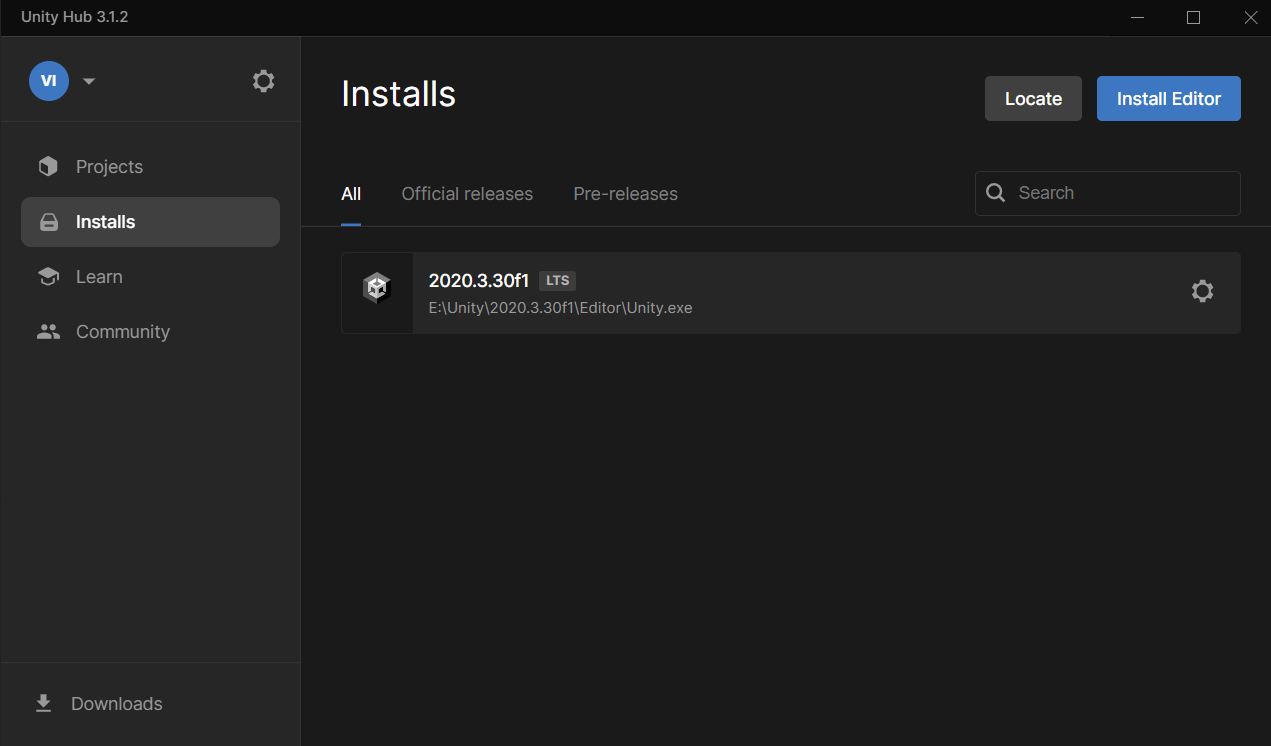
\includegraphics[width=\textwidth]{img/hub1.PNG}
\caption{Instalación Editor Unity 1 }
\end{figure}

Llegados a este punto seleccionando en instalar editor nos aparecerá la siguiente ventana que nos permitirá seleccionar la versión del editor que queramos utilizar. Recomiendo para el uso de este proyecto la versión 2020.3.30f1 ya que es con el que ha sido desarrollado y el cambio de versiones de editor puede acarrear fallos o problemas inesperados.


\begin{figure}[h]
\centering
\label{Instalación Editor Unity 2}
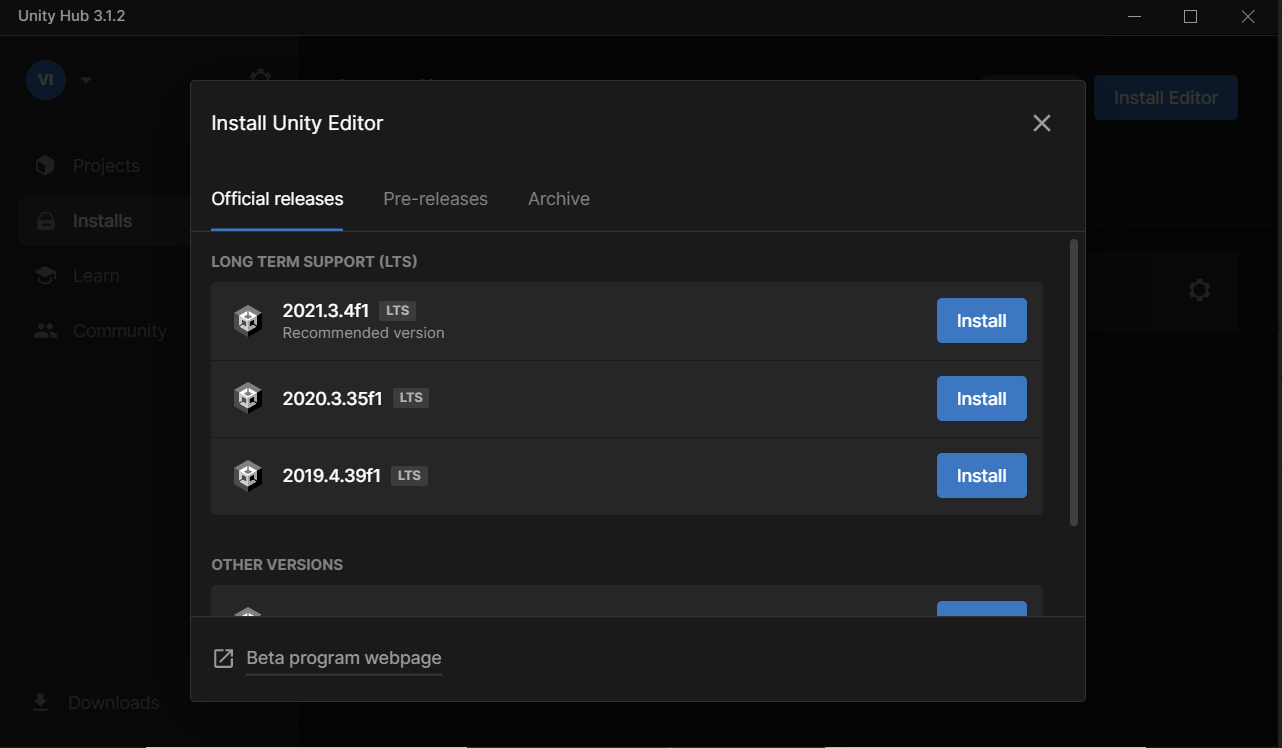
\includegraphics[width=\textwidth]{img/hub2.PNG}
\caption{Instalación Editor Unity 2}
\end{figure}


\newpage


\newpage
\subsubsection{Componentes Software}
Para poder hacer uso de nuestros dispositivos de realidad virtual necesitaremos del software especializado requerido. Por ello aquí veremos qué necesitamos instalar en nuestro ordenador.
\begin{itemize}
    \item \textbf{SenseCom}:
    Este software es el necesario de instalar para poder utilizar nuestros guantes hápticos, para ello nos dirigiremos a la página web de \textit{senseglove.com} y accederemos al apartado de developers. Desde ese apartado podremos adentrarnos en el proyecto de GitHub SenseGlove-API, el cual contiene un ejecutable que instalará este software.
    
    Se muestra a continuación una imagen del contenido de lo descargado junto a la pantalla de instalación, tras ejecutar el instalador.
    
    \begin{figure}[h]
\centering
\label{Instalación Software SenseGlove}
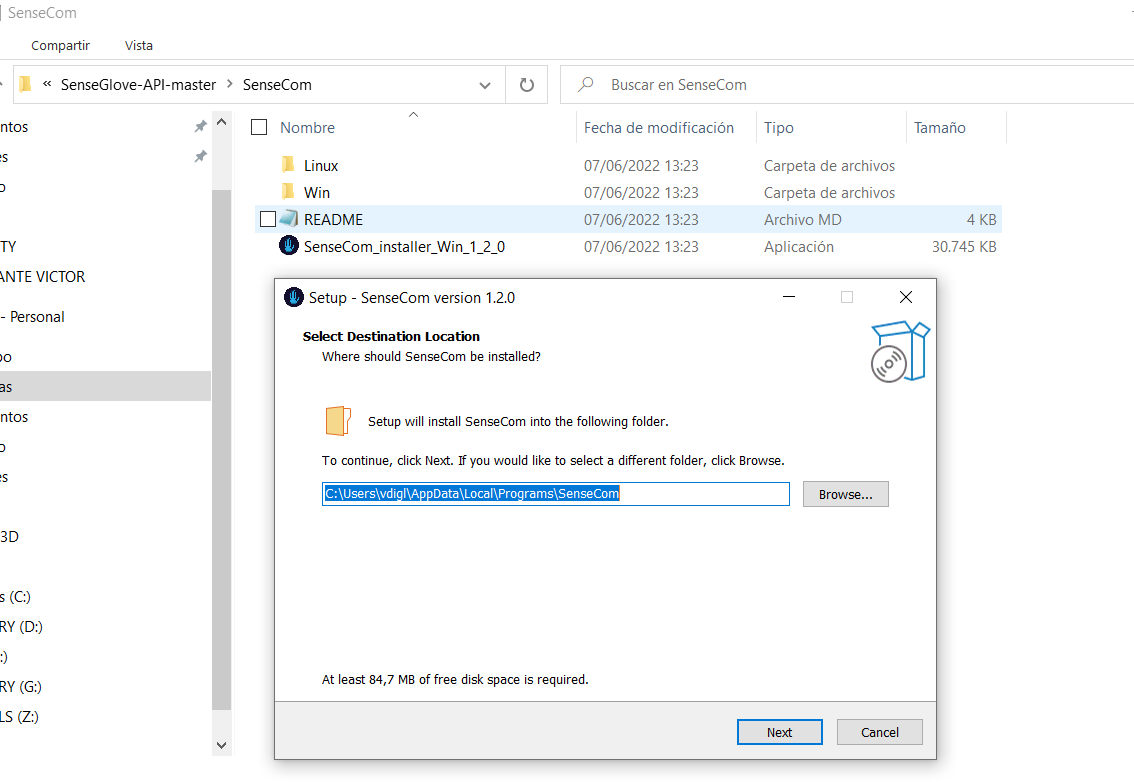
\includegraphics[width=1.1\textwidth]{img/sensecom01.PNG}
\caption{Instalación Software SenseGlove}
\end{figure}

\newpage
\item \textbf{Oculus}:
El siguiente software que debemos instalar en nuestro PC es el de Oculus\cite{Quest2} ya que sin el, no podremos conectar nuestro dispositivo Oculus Quest 2 ni sus controladores a Unity. 
Para esta instalación, accederemos a la siguiente página web => \textit{https://store.facebook.com/es/quest/setup/} y descargaremos el software.

En este punto se nos descargará un archivo \textit{OculusSetup.exe}, el cual debemos ejecutar, y tras revisar los términos y condiciones nos aparecerá la siguiente pantalla:

    \begin{figure}[h]
\centering
\label{Instalación Software Oculus}
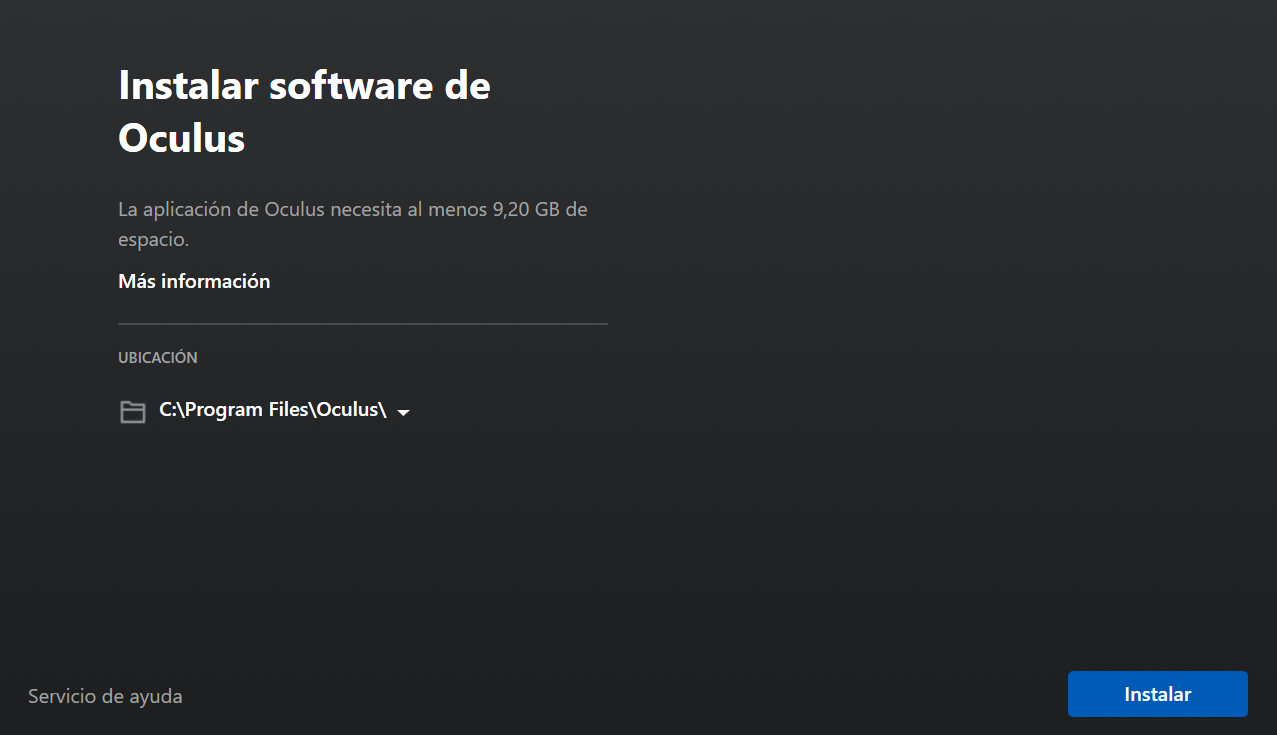
\includegraphics[width=1.1\textwidth]{img/oculus.PNG}
\caption{Instalación Software Oculus}
\end{figure}

\newpage
Tras realizar la instalación se nos requerirá de la creación de una cuenta que puede ser de \textit{Facebook} y posteriormente a todo este proceso, ya podremos configurar nuestro hardware y simplemente con tener las gafas conectadas al PC podremos usar los dispositivos desde Unity.

\item \textbf{IP Advanced Scanner}: Para descargar este software, que nos servirá de gran ayuda a la hora de preparar la conexión con nuestro robot debemos acceder a la web oficial que es la siguiente=> \textit{https://www.advanced-ip-scanner.com/es/} y realizar la descarga. Este software está configurado para poder instalarse en el ordenador o para ser ejecutado de manera única con su versión portátil.

Al correr el ejecutable se nos abre la siguiente ventana que nos permite elegir:

    \begin{figure}[h]
\centering
\label{Instalación Escáner de RED}
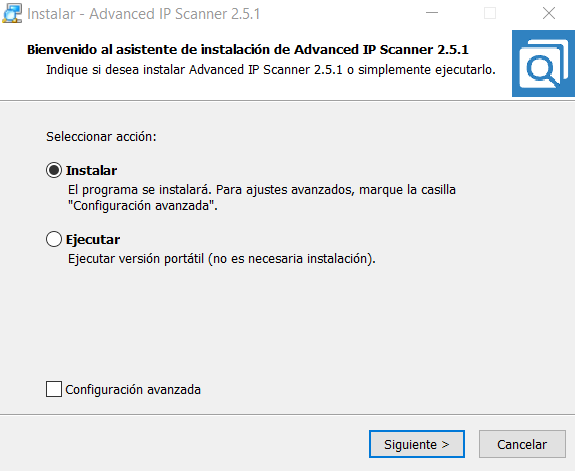
\includegraphics[width=0.9\textwidth]{img/ipad.PNG}
\caption{Instalación Escáner de RED}
\end{figure}

\newpage
Una vez aquí podemos seleccionar la opción que prefiramos, en caso de de instalar, seleccionaremos la ruta de destino de la instalación y ya tendríamos este software.

\end{itemize}


\newpage
\section{Compilación, instalación y ejecución del proyecto}
Llegados a este punto del anexo, en caso de querer utilizar el proyecto, deberíamos tener instaladas ya las aplicaciones comentadas previamente.
Ahora bien, comenzaremos con la compilación, instalación y forma de ejecutar este proyecto.

En primer lugar tendremos que comprobar tres cosas:
\begin{enumerate}
    \item Comprobar con SenseCom que tenemos conexión con los guantes, para ello debemos de tenerlos encendidos y añadidos a dispositivos bluetooth de nuestro PC. Tras esto, al abrir el software nos saldrá en pantalla que se encuentran conectados y veremos una representación de nuestras manos.
    \item Comprobar la conexión de Oculus con su software, se puede conectar vía WIFI o lo recomendado por cable, ya que la conexión es directa.
    \item Comprobar con el escáner de red instalado, la dirección IP del robot.
\end{enumerate}

Los siguientes pasos son ya relacionados con Unity.
\newpage
\subsection{Unity}
Abrimos Unity Hub y seleccionaremos el botón de \textit{Open} ya que es el que nos permite añadir proyectos a nuestro Unity. 

   \begin{figure}[h]
\centering
\label{Importar Proyecto}
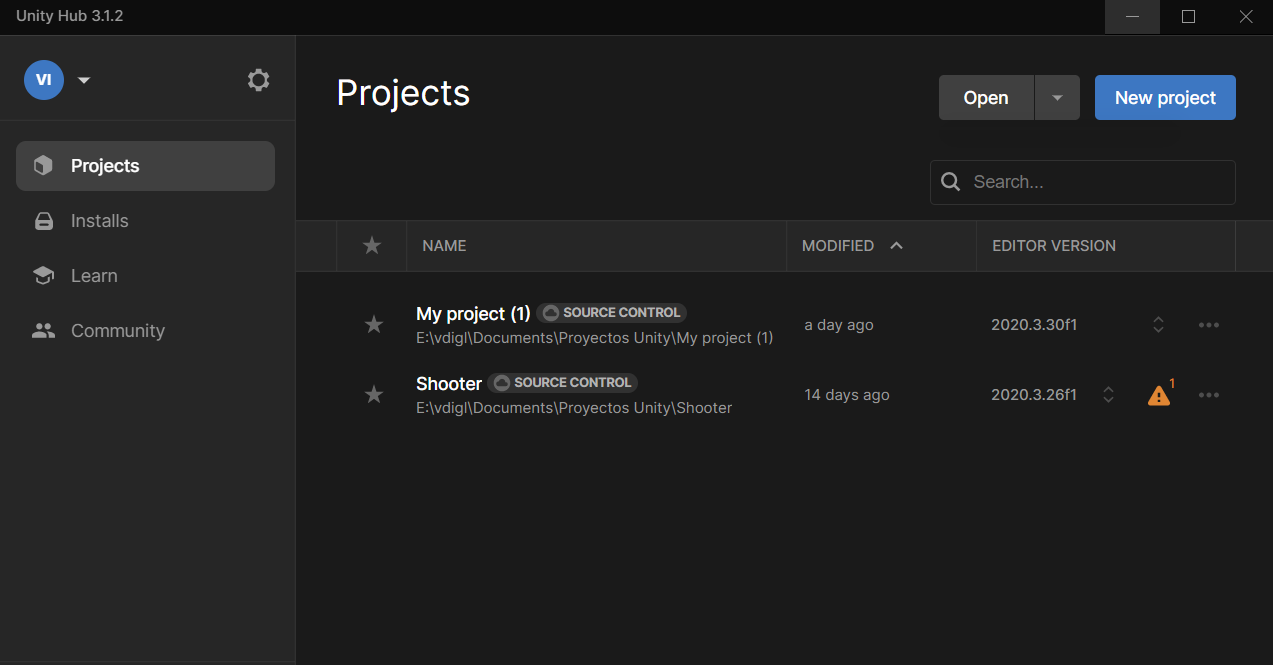
\includegraphics[width=0.9\textwidth]{img/hub3.PNG}
\caption{Importar Proyecto}
\end{figure}

Después de esto se nos abrirá la clásica ventana de nuestro explorador que nos permitirá llegar al punto donde tengamos la carpeta del proyecto, para así poder abrirlo e importarlo. Deberemos seleccionar de las versiones del editor que tengamos instaladas la que queramos utilizar para este proyecto. La recomendada por mi es la \textit{2020.3.30f1}

Recuerdo de nuevo que se recomienda siempre utilizar la versión del editor correspondiente a la de quién realizó el proyecto, ya que pueden aparecer errores o problemas de importación.

\newpage
Una vez tengamos todo importado, en la parte baja de la pantalla aparece el explorador de Unity y accedemos dentro de la carpeta \textit{Assets} a la carpeta de nombre \textit{Scenes}. Posteriormente debemos seleccionar la escena \textit{Ros} ya que es el software final del proyecto.

   \begin{figure}[h]
\centering
\label{Explorador archivos de proyecto}
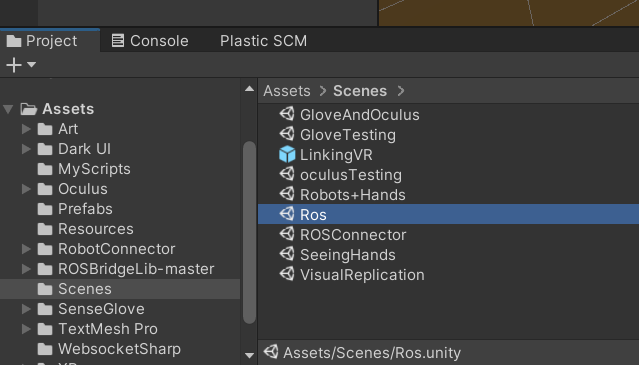
\includegraphics[width=0.9\textwidth]{img/inst1.PNG}
\caption{Explorador archivos de proyecto}
\end{figure}

Una vez abierta esta escena en la parte superior izquierda de la pantalla, nos aparecerá una jerarquía con los \textit{GameObjects}\cite{GameObjects} de nuestra escena. Debemos de seleccionar \textit{ROSInitializer} para configurar la conexión. En el lado derecho en el \textit{Inspector} nos aparecerá el siguiente cuadro: 

   \begin{figure}[h]
\centering
\label{Configuración de conexión con Robot}
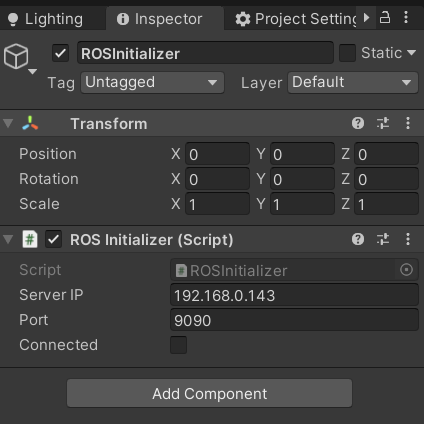
\includegraphics[width=0.45\textwidth]{img/inst2.PNG}
\caption{Configuración de conexión con Robot}
\end{figure}

En este cuadro tendremos que rellenar con el número de IP y el puerto para que a la hora de ejecutar sea capaz de conectar con el robot. El resto de los valores asociados a cada variable o componente de los \textit{GameObjects} de esta escena se deben de mantener igual.

Con todo esto ya tendremos listo el software para llevar a cabo la \textit{build} y empezar a usarlo.
Para ello en la barra superior de herramientas accedemos a => \textit{File}->\textit{Build Settings} y se nos mostrará la siguiente ventana:

   \begin{figure}[h]
\centering
\label{Realizando \textit{Build} del proyecto}
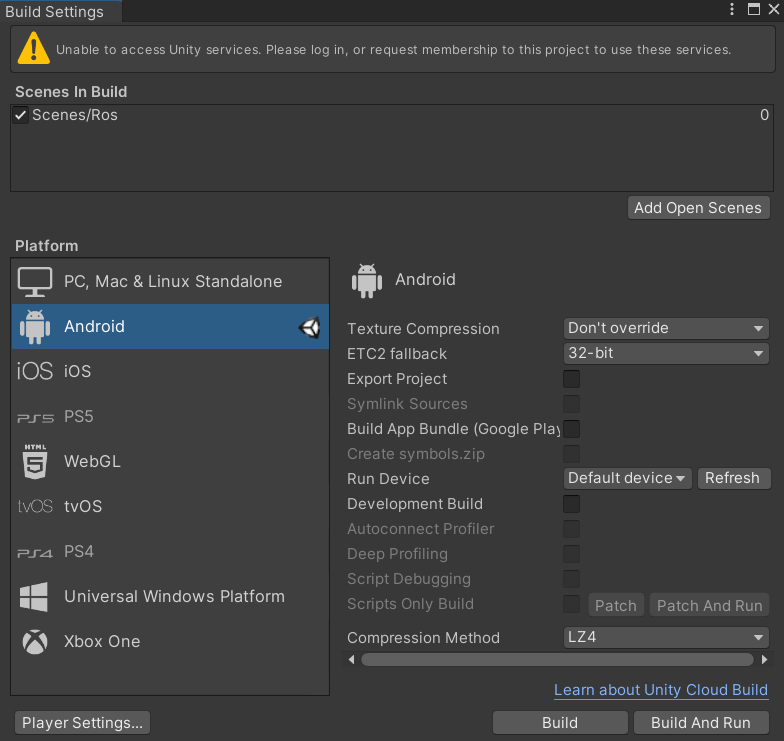
\includegraphics[width=0.8\textwidth]{img/inst3.PNG}
\caption{Realizando \textit{Build} del proyecto}
\end{figure}

En el apartado \textit{Run Device} debemos o dejarlo en dispositivo por defecto o seleccionar el dispositivo Android VR\cite{VR} (Las Oculus Quest 2 en mi caso) que queramos utilizar con Unity.
Seleccionamos \textit{Build} y se abrirá un explorador de archivos que nos permitirá alojar nuestro archivo \textit{.apk} que correremos en el dispositivo Android.

\newpage
En caso correcto, en la carpeta de destino seleccionada debemos ver el siguiente fichero .apk con el nombre seleccionado (En este caso \textit{Build1.apk}).
   \begin{figure}[h]
\centering
\label{Realizando la \textit{Build} resultante de proyecto}
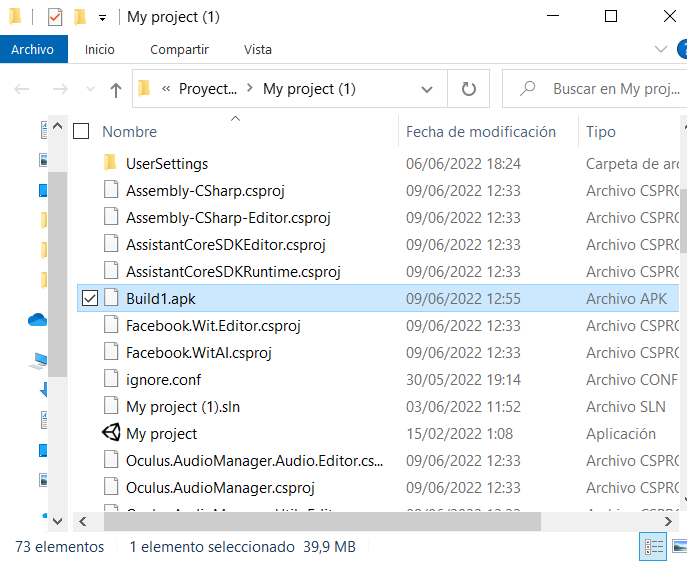
\includegraphics[width=0.8\textwidth]{img/inst4.PNG}
\caption{Realizando \textit{Build} resultante de proyecto}
\end{figure}

A partir de aquí, si tenemos conectados todos los dispositivos, solo nos quedaría pulsar el botón \textit{Run/Play} de Unity para que se ejecute el proyecto y comenzar a trabajar junto al robot y demás dispositivos.

